\chapter{Reinforcement Learning Model}
\label{chap:RLModel}
\section{Introduction}
In the last session we analyzed the task-related activity patterns of principal assembly-pair types.\\Significant task related activity was tested with Friedman test in stimulus presentation (CS+/-) interval, stimulus continued\footnote{The window right before the reward delivery time, or the expected reward time in False Alarm trials, or the hypothetical reward time in Correct Rejection trials.} (CS+/- cont.) interval, and reward\footnote{Or expected reward in False Alarm trials, or Hypothetical Reward in Correct Rejection trials.}.\\We found a good portion of SPN-DAN pairs becoming active early at stimulus presentation, another important group being active later during the stimulus presentation, and only a small fraction of SPN-DAN pairs active only at the retrieval.\\The described activity pattern makes SPN-DAN pairs good candidates for reward prediction (RP) coding.\\On the other hand we observed that FSN-DAN pairs are early activated by the stimulus on onset and they show as well a phasic activity at the reward time.\\This kind of activity pattern suggests that FSN-DAN pairs could code for reward prediction error (RPE).\\However we are not able to address those question with the presented activity patterns description, that is rather static, whereas the performed task was highly dynamic.\\The task was such that the animal had to assign and re-assign a value to the rewarded odor to be able to predict the reward.\\To take into account the learning dynamic, we used the reinforcement learning technique \cite{SuttonBarto}. $"$Reinforcement learning$"$ is an area in machine learning, in which an agent tries to learn the best action to take, depending on the circumstances in which this action will be performed, this approach can incorporate any changes in the environment of the decision making process. In psychology, from where the idea of this machinery derives, the concept is known as “learning by reinforcement”: the agent receives a reward or punishment, depending on the decision made, through the experience he is able to associate the actions that generate the greatest reward for each situation that the environment presents, and to avoid unrewarded actions or actions that generate punishment.\\
Machine learning uses the same idea: the machine observes a state and, based on this, chooses an action to take and receives the reward associated with that specific action in that state, thus obtaining the information of this specific combination. The process is repeated until the machine is able to choose the best action to take for each of the possible scenarios to be observed in the future.\\In the contingencies of the experiment conducted in our lab, two odor were presented and only one was associated with a reward with a probability of 0.9. Each time one odor was presented the mouse chose to take the action (lick or not lick) that maximized the reward and minimized his effort. the task was learnt when the animal was able to lick for the rewarded odor and not lick when the unrewarded odor was presented.\\To model this learning process we set up a Rescorla Wagner model with Pearce Hall update mechanism (\cite{Li}, \cite{Costa}, \cite{Koppe}).\\

%%
%We use here Reinforcement Learning/Forgetting models (\cite{SuttonBarto}) with Q-learning values (\cite{Dayan1}) to fit mice behaviour in go-no go odor discrimination task; we regress afterwards neuronal activity with model values.
\section{Model}
%%%%%{\color{blue}Start writing equation of reinforcement learning}
%%%%%First Option I tried, Georgia's option {\color{red}cite Georgia's paper}
%%%%%We set up four RL models and we chose the one that better fitted the behaviour for the regression analysis.
Reinforcement learning model are usually set up as follows:
\begin{itemize}
    \item At each trial $t$ of the experiment, a state $s$ is observed, this is an input of the model.
    \item After the stimulus presentation, the animal has the chance to take an action, and according to choice made, the reward is delivered. The reward is a vector $r(t)$, each vector component indicates the reward value delivered at the trial $t$, the reward vector is an input of the model.
    \item After the reward delivery, the animal computes the reward prediction error, that is evaluated in the model as the difference between the actual reward and the expected reward.
    \item States values are the expected reward values and they are updated according to the last expected values and the reward prediction error and it is modulated by the learning rate.
    \item The learning rate is often a constant free parameter, however it has been shown that a time dependent variable better describes the learning dynamic (\cite{Funamizu}, \cite{Daw}).
    \item Learned values are then translated into action probabilities via a softmax function, maximized with respect some free parameters.
\end{itemize}
We set up an hybrid Rescorla-Wagner/Pearce-Hall update mechanism following the scheme above.
The V values are updated according to the equation
\begin{equation}
V_s(t+1)=V_s(t)+k\cdot\alpha(t)\cdot\delta  \hspace{0.3cm} with \hspace{0.3cm}\delta(t)=r(t)-V_s(t)
\label{VValues}
\end{equation}
where $\delta$ is the prediction error. Importantly V values are modulated according to the time dependent learning component $\alpha(t)$, this component is directly related to the uncertainty to get the reward. The need to introduce a time dependent learning rate was emphasized first in works as \cite{Daw} and \cite{Funamizu}.
\begin{figure}
    \centering
    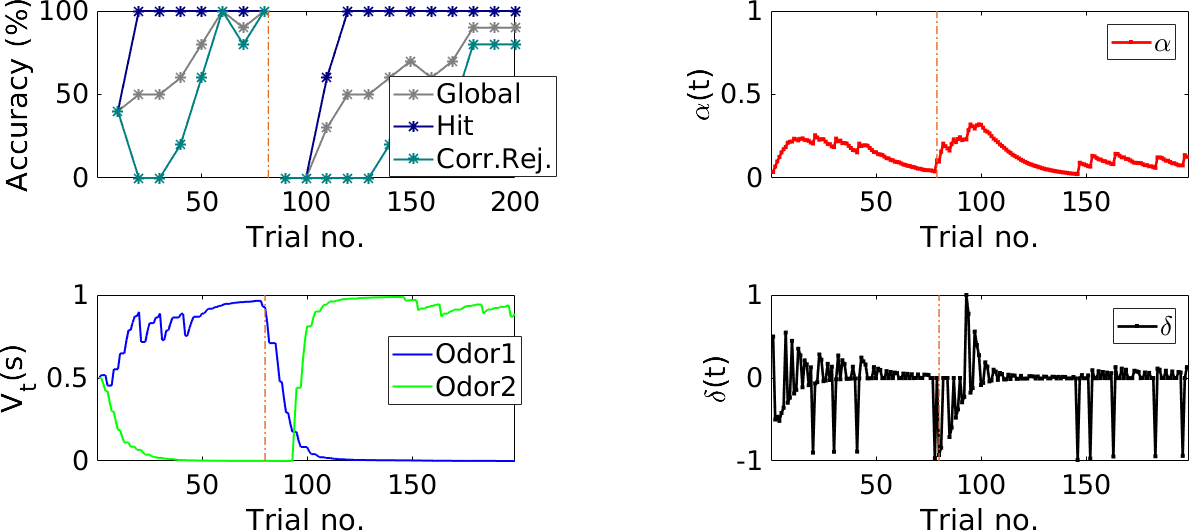
\includegraphics[scale=0.45]{figures/Lastrev1_V05_An6.png}
    \caption{Caption}
    \label{fig:RL_ex}
\end{figure}
